%% beamer packages
% other themes: AnnArbor, Antibes, Bergen, Berkeley, Berlin, Boadilla, boxes, 
% CambridgeUS, Darmstadt, Dresden, Frankfurt, Goettingen, Hannover, Ilmenau,
%JuanLesPins, Luebeck, Madrid, Malmoe, Marburg, Montpellier, PaloAlto,
%Pittsburgh, Rochester, Singapore, Szeged, Warsaw
% other colors: albatross, beaver, crane, default, dolphin, dove, fly, lily, 
%orchid, rose, seagull, seahorse, sidebartab, structure, whale, wolverine,
%beetle

%\documentclass[xcolor=dvipsnames]{beamer}
\documentclass[table,dvipsnames]{beamer}
\usepackage{beamerthemesplit}
\usepackage{bm,amsmath,marvosym}
\usepackage{listings,color}%xcolor
\usepackage[ngerman]{babel}
\usepackage{natbib}
\usepackage{media9}
\usepackage[utf8]{inputenc}
\definecolor{shadecolor}{rgb}{.9, .9, .9}
\definecolor{darkblue}{rgb}{0.0,0.0,0.5}
\definecolor{myorange}{cmyk}{0,0.7,1,0}
\definecolor{mypurple}{cmyk}{0.3, 0.9, 0.0, 0.2}

% make a checkmark
\usepackage{tikz}
\def\checkmark{\tikz\fill[scale=0.4](0,.35) -- (.25,0) -- (1,.7) -- (.25,.15) -- cycle;} 

% dot product
\usetikzlibrary{arrows,positioning}
\tikzset{
    %Define standard arrow tip
    >=stealth',
    % Define arrow style
    pil/.style={->,thick}
}

% math stuff
\newcommand{\argmin}{\operatornamewithlimits{argmin}}

\lstnewenvironment{code}{
    \lstset{backgroundcolor=\color{shadecolor},
        showstringspaces=false,
        language=python,
        frame=single,
        framerule=0pt,
        keepspaces=true,
        breaklines=true,
        basicstyle=\ttfamily,
        keywordstyle=\bfseries,
        basicstyle=\ttfamily\scriptsize,
        keywordstyle=\color{blue}\ttfamily,
        stringstyle=\color{red}\ttfamily,
        commentstyle=\color{green}\ttfamily,
        columns=fullflexible
    }
}{}

\lstnewenvironment{codeout}{
    \lstset{backgroundcolor=\color{shadecolor},
        frame=single,
        framerule=0pt,
        breaklines=true,
        basicstyle=\ttfamily\scriptsize,
        columns=fullflexible
    }
}{}

\hypersetup{colorlinks = true, linkcolor=darkblue, citecolor=darkblue,urlcolor=darkblue}
\hypersetup{pdfauthor={A. Richards}, pdftitle={Multi-armed Bandit}}

\newcommand{\rd}{\textcolor{red}}
\newcommand{\grn}{\textcolor{green}}
\newcommand{\keywd}{\textcolor{myorange}}
\newcommand{\highlt}{\textcolor{NavyBlue}}
\newcommand{\norm}[1]{\left\lVert#1\right\rVert}
\def\ci{\perp\!\!\!\perp}
% set beamer theme and color
\usetheme{Frankfurt}
%\usetheme{Berkeley}
\usecolortheme{orchid}
%\usecolortheme{seagull}


%% fix the section title for literature
\renewcommand{\bibsection}{\subsubsection*{\bibname } }

\title[Bayesian A/B]{Multi-armed Bandit}
\author[A. Richards]{A. Richards}
\institute{}
\date[]{02.08.2017}

%%%%%%%%%%%%%%%%%%%%%%%%%%%%%%%%%%%%%%%%%%%%%%%%%%%%%%%%%%%%%%%%%%%%%%%%%%%%%%%
\begin{document}
\frame{\titlepage}
%%%%%%%%%%%%%%%%%%%%%%%%%%%%%%%%%%%%%%%%%%%%%%%%%%%%%%%%%%%%%%%%%%%%%%%%%%%%%%%
\frame{
\footnotesize
\tableofcontents
\normalsize
}

%%%%%%%%%%%%%%%%%%%%%%%%%%%%%%%%%%%%%%%%%%%%%%%%%%%%%%%%%%%%%%%%%%%%%%%%%%%%%%%
\section{A/B frameworks}
\subsection{}

%%%%%%%%%%%%%%%%%%%%%%%%%%%%%%%%%%%%%%%%%%%%%%%%%%%%%%%%%%%%%%%%%%%%%%%%%%%%%%%
\frame{   
\frametitle{Objectives}
\begin{block}{Morning}
 \begin{itemize}
  \item Overview of Frequentist A/B testing
  \item Overview of Bayesian A/B testing
  \item Review of Bayes’ Theorem 
  \item Conjugate Priors
  \item Is CTR$_{A}$ is better than CTR$_B$ through Code
  \end{itemize}
\end{block}
}

%%%%%%%%%%%%%%%%%%%%%%%%%%%%%%%%%%%%%%%%%%%%%%%%%%%%%%%%%%%%%%%%%%%%%%%%%%%%%%%
\frame{   
\frametitle{Frequentist A/B testing}
\footnotesize

\begin{enumerate}
 \item define a metric
 \item determine parameters of interest for study (number of observations, 
power, significance threshold, and so on)
 \item run test, without checking results, until number of observations has
been achieved
 \item calculate p-value associated with hypothesis test
 \item report $p$-value and suggestion for action
\end{enumerate}
}

%%%%%%%%%%%%%%%%%%%%%%%%%%%%%%%%%%%%%%%%%%%%%%%%%%%%%%%%%%%%%%%%%%%%%%%%%%%%%%%
\frame{   
\frametitle{Bayesian A/B testing}
\footnotesize
\begin{enumerate}
 \item Define a metric
 \item Run test, continually monitor results
 \item At any time calculate probability that $A \geq B$ or vice versa
 \item Suggest course of action based on probabilities calculated
\end{enumerate}
}

%%%%%%%%%%%%%%%%%%%%%%%%%%%%%%%%%%%%%%%%%%%%%%%%%%%%%%%%%%%%%%%%%%%%%%%%%%%%%%%
\frame{   
\frametitle{Discussion}

Obtaining significance depends on \highlt{power}

\begin{block}{}
 \begin{itemize}
  \item What are the factors that influence power?
  \item Which A/B testing framework relies on significance testing?
  \item What about the other framework what does it use to guide decisions?
  \end{itemize}
\end{block}

With the Bayesian framework you:
\begin{itemize}
 \item have a degree of Belief?
 \item can say \textit{it is 95\% likely that site A is better than site B}?
 \item can stop a test early based on surprising data
\end{itemize}
}

%%%%%%%%%%%%%%%%%%%%%%%%%%%%%%%%%%%%%%%%%%%%%%%%%%%%%%%%%%%%%%%%%%%%%%%%%%%%%%%
\frame{ 
\frametitle{That formula again}
\footnotesize
\begin{equation}
P(\theta|y) = \frac{P(y|\theta)P(\theta)}{P(y)}
\end{equation}

\begin{itemize}
 \item \keywd{prior} - $P(\theta)$ - one's beliefs about a quantity before 
presented with evidence
 \item \keywd{posterior} - $P(\theta|y)$ - probability of the parameters given 
the evidence
 \item \keywd{likelihood} - $P(y|\theta)$  - probability of the evidence given 
the parameters
 \item \keywd{normalizing constant} - $P(y)$
\end{itemize}
}

%%%%%%%%%%%%%%%%%%%%%%%%%%%%%%%%%%%%%%%%%%%%%%%%%%%%%%%%%%%%%%%%%%%%%%%%%%%%%%%
\section{Priors}
\subsection{}

%%%%%%%%%%%%%%%%%%%%%%%%%%%%%%%%%%%%%%%%%%%%%%%%%%%%%%%%%%%%%%%%%%%%%%%%%%%%%%%
\begin{frame}[fragile]
\frametitle{Lets talk about priors}
\footnotesize

\begin{block}{Subjective vs Objective priors}
Bayesian priors can be classified into two classes: \keywd{objective priors}, 
which aim to allow the data to influence the posterior the most, and 
\keywd{subjective priors}, which allow the practitioner to express his or her 
views into the prior.
\end{block}

\begin{itemize}
 \item If we added more probability mass to certain areas of 
the prior, and less elsewhere, we are biasing our inference towards the 
unknowns 
existing in the former area.
\item The prior's influence changes as our dataset increases
\end{itemize}
\end{frame}

%%%%%%%%%%%%%%%%%%%%%%%%%%%%%%%%%%%%%%%%%%%%%%%%%%%%%%%%%%%%%%%%%%%%%%%%%%%%%%%
\frame{
\begin{block}{Empirical Bayes}
It is not a true Bayesian method. Empirical Bayes combines frequentist and 
Bayesian inference.  The prior distribution, instead of being selected 
beforehand is estimated directly from the data generally with frequentist 
methods.
\end{block}
\vspace{0.5cm}
\href{https://en.wikipedia.org/wiki/Empirical\_Bayes\_method}{
https://en.wikipedia.org/wiki/Empirical\_Bayes\_method}
\vspace{0.5cm}
\begin{block}{CAUTION}
 Many people feel that empirical bayes is \textit{double counting} or 
\textit{double dipping} from the data
\end{block}
}

%%%%%%%%%%%%%%%%%%%%%%%%%%%%%%%%%%%%%%%%%%%%%%%%%%%%%%%%%%%%%%%%%%%%%%%%%%%%%%%
\frame{
\frametitle{The Gamma distribution}
\scriptsize
A Gamma random variable, denoted $X \sim \text{Gamma}(\alpha, \beta)$, is 
also

\begin{equation}
\text{Exp}(\beta) \sim \text{Gamma}(1, \beta)
\end{equation}

The additional parameter gives flexibility which helps us better express
subjective priors. The density function for a $\text{Gamma}(\alpha, \beta)$ 
random variable is:

\begin{equation}
f(x \mid \alpha, \beta) = \frac{\beta^{\alpha}x^{\alpha-1}e^{-\beta 
x}}{\Gamma(\alpha)} 
\end{equation}

where $\Gamma(\alpha)$ is the 
\href{http://en.wikipedia.org/wiki/Gamma\_function)}{Gamma 
function}

\begin{center}
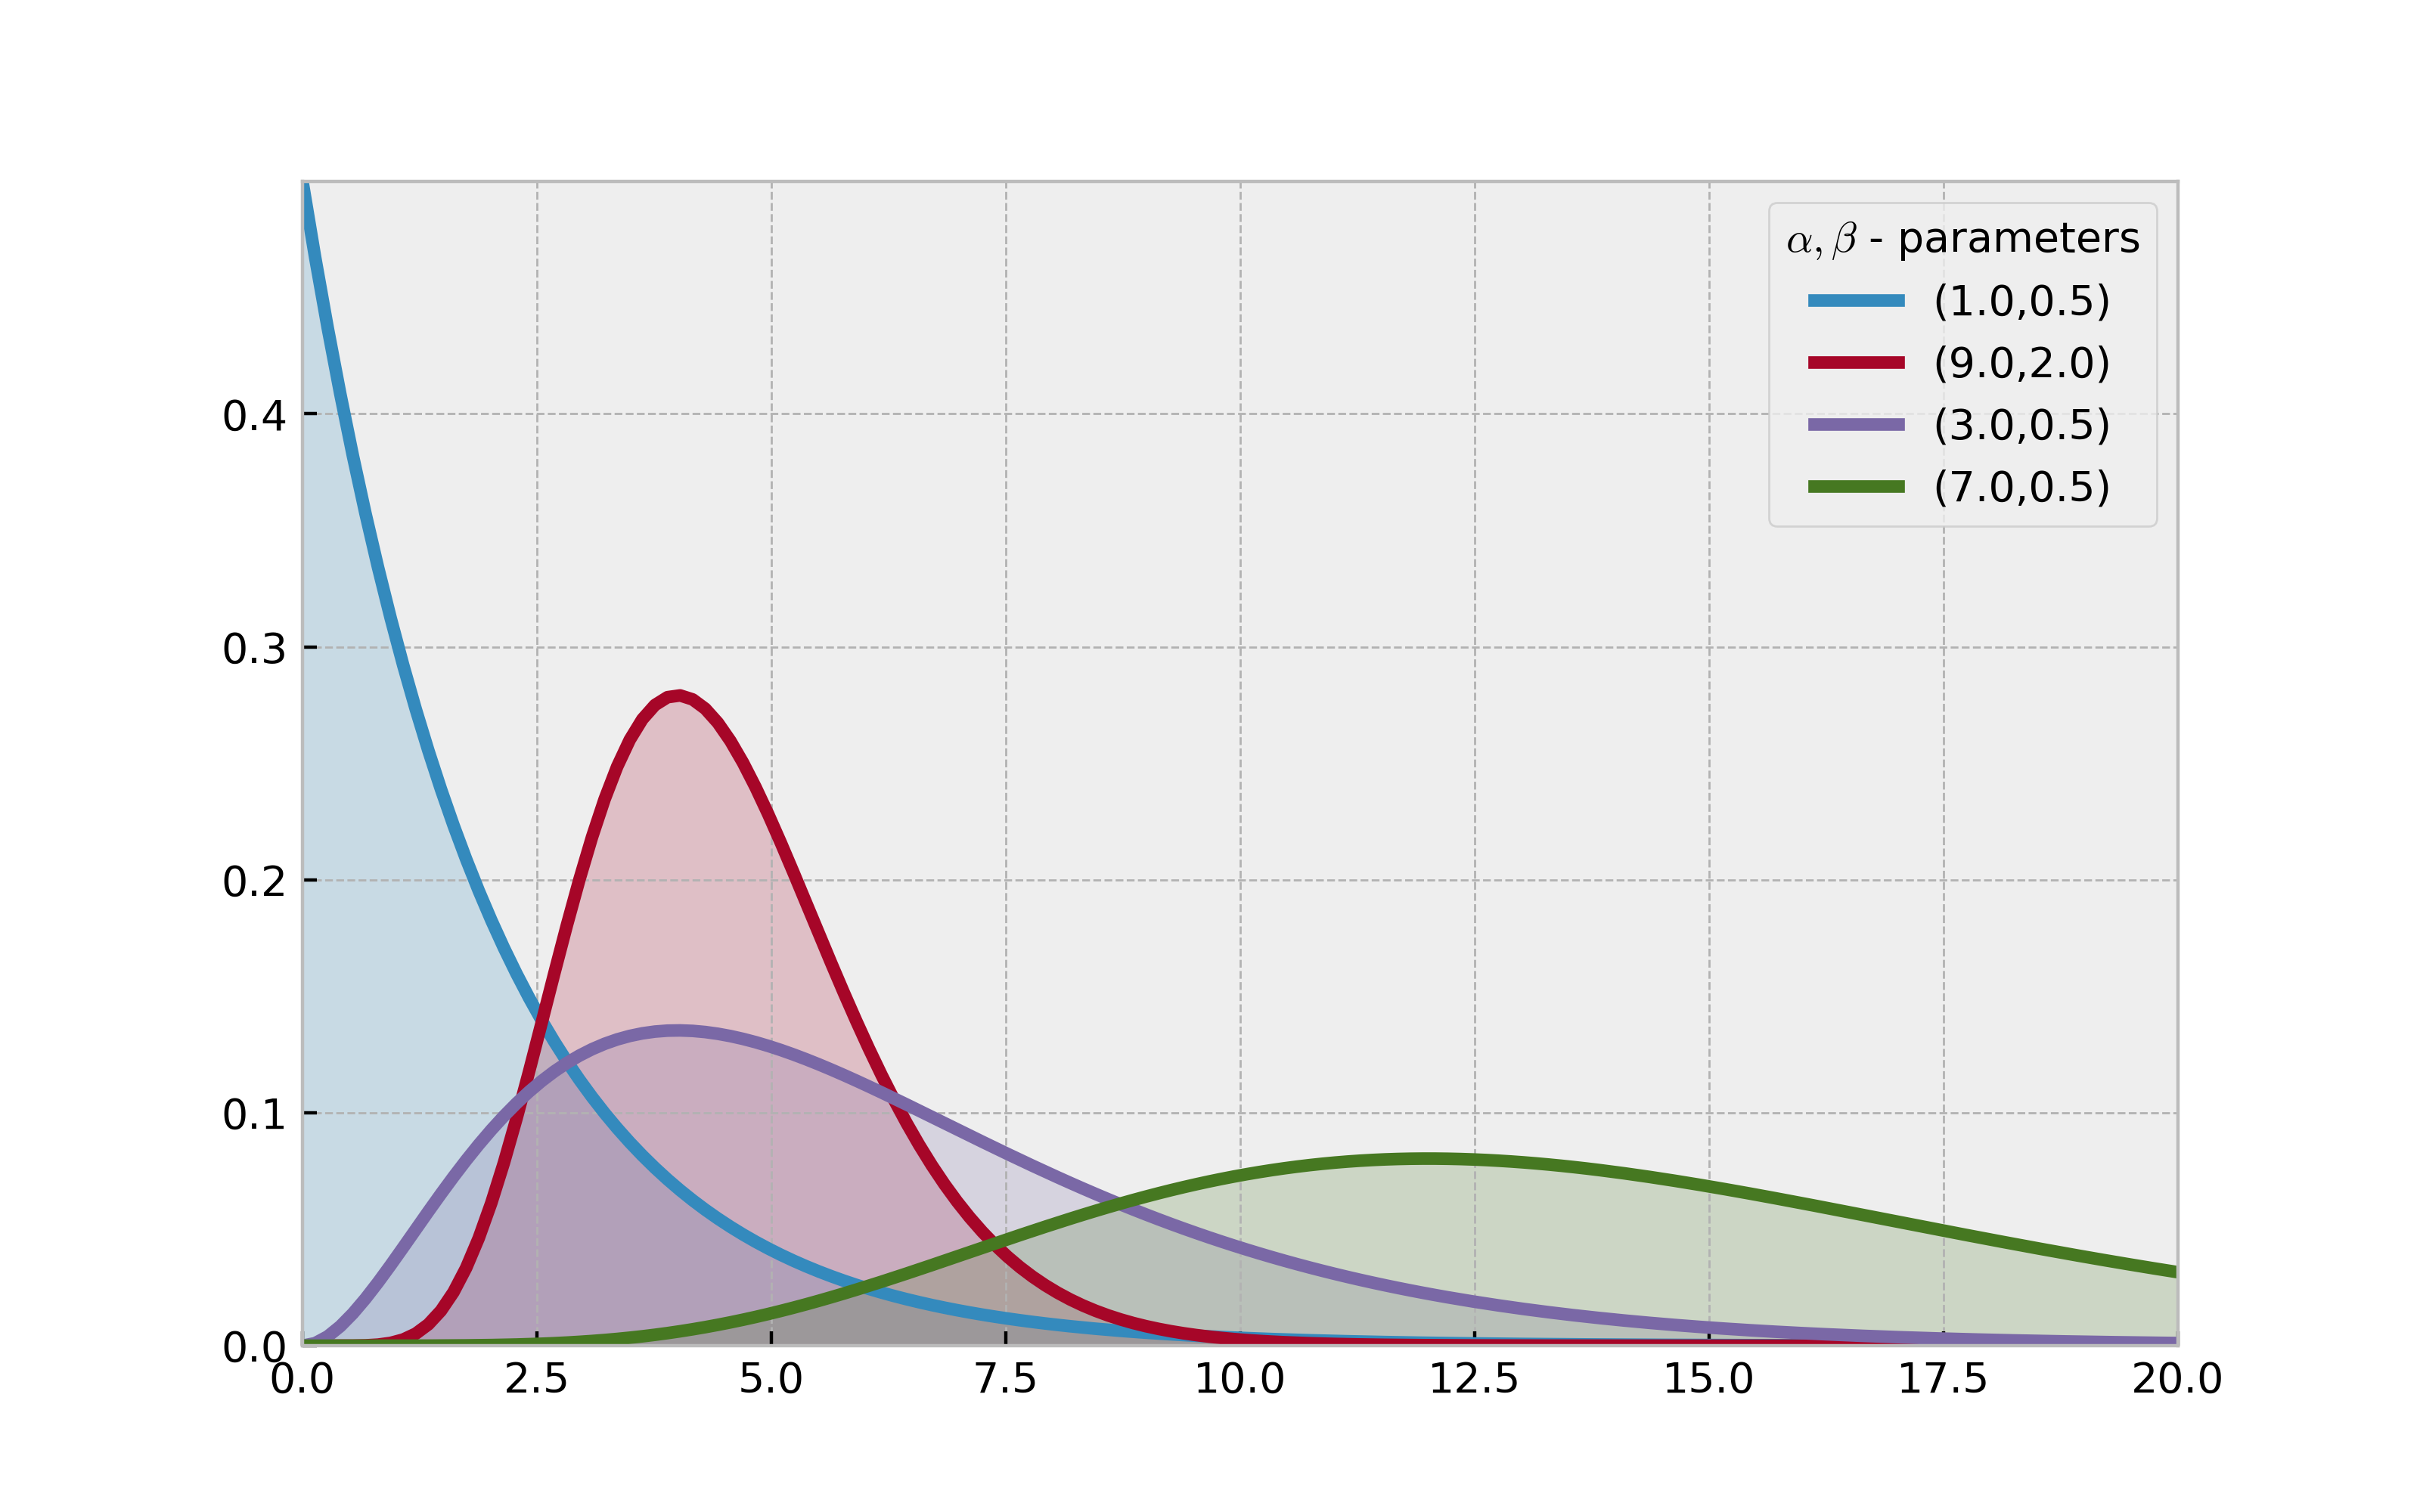
\includegraphics[scale=0.32]{gamma-priors.png}
\end{center}

\begin{flushleft}
 
\tiny{\href{
http://nbviewer.jupyter.org/github/CamDavidsonPilon/Probabilistic-Programming-an
d-Bayesian-Methods-for-Hackers/blob/master/Chapter6\_Priorities/Ch6\_Priors\_PyM
C 2 . ipynb}{Bayesian methods for hackers (chap 6)}}
\end{flushleft}

}

%%%%%%%%%%%%%%%%%%%%%%%%%%%%%%%%%%%%%%%%%%%%%%%%%%%%%%%%%%%%%%%%%%%%%%%%%%%%%%%
\frame{
\frametitle{The Beta distribution}
\footnotesize

The Beta distribution is very useful in Bayesian statistics. A random variable 
$X$ has a $\text{Beta}$ distribution, with parameters $(\alpha, \beta)$, if its 
density function is:

\begin{equation}
f_X(x | \; \alpha, \beta ) = \frac{ x^{(\alpha - 1)}(1-x)^{ (\beta - 1) } 
}{B(\alpha, \beta) }
\end{equation}

where $B$ is the \href{http://en.wikipedia.org/wiki/Beta\_function}{Beta 
function} (hence the name). The random variable $X$ is only allowed in [0,1], 
making the Beta distribution a popular distribution for decimal values, 
probabilities and proportions. The values of $\alpha$ and $\beta$, both positive 
values, provide great flexibility in the shape of the distribution.

\begin{center}
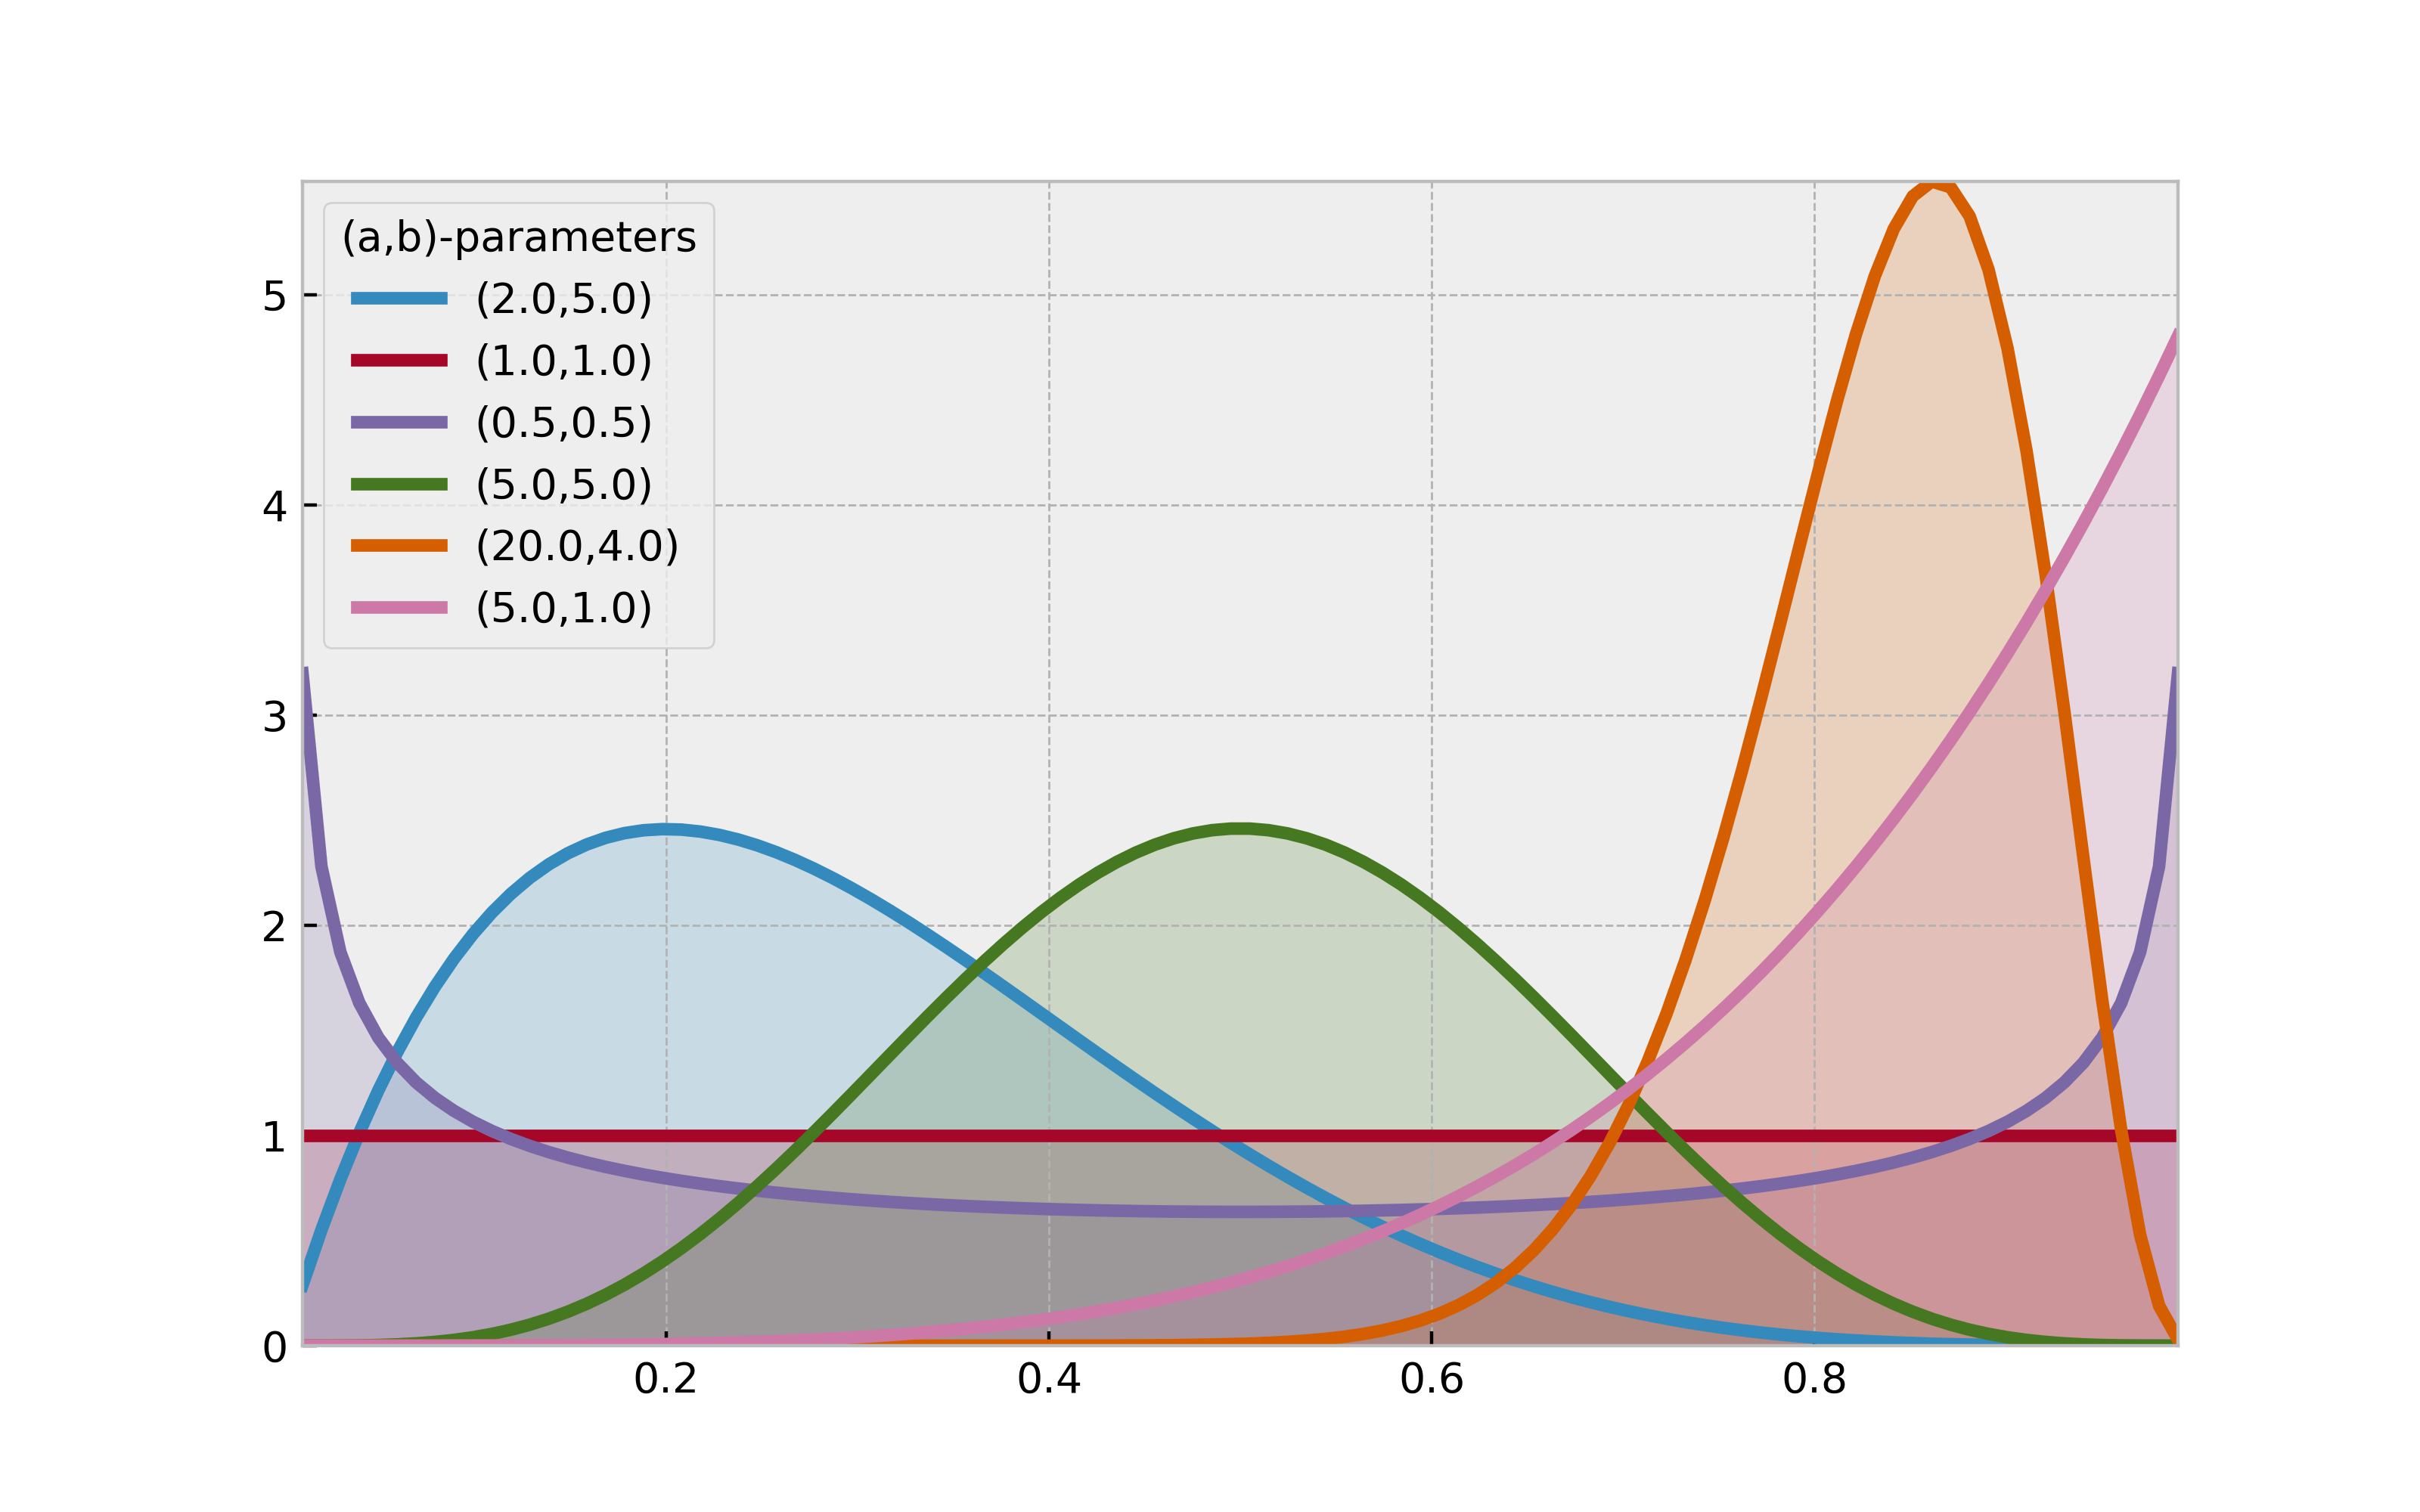
\includegraphics[scale=0.32]{beta-priors.png}
\end{center}

% \begin{flushleft}
% \tiny{\href{
% http://nbviewer.jupyter.org/github/CamDavidsonPilon/Probabilistic-Programming-an
% d-Bayesian-Methods-for-Hackers/blob/master/Chapter6\_Priorities/Ch6\_Priors\_PyM
% C 2.ipynb}{Bayesian methods for hackers (chap 6)}}
% \end{flushleft}
}

%%%%%%%%%%%%%%%%%%%%%%%%%%%%%%%%%%%%%%%%%%%%%%%%%%%%%%%%%%%%%%%%%%%%%%%%%%%%%%%
\frame{
\frametitle{So what?}
\footnotesize
There is an interesting connection between the Beta distribution and the 
Binomial distribution. Suppose we are interested in some unknown proportion or 
probability $p$. (think of coin example)
\vspace{0.5cm}
\begin{itemize}
 \item We assign a $\text{Beta}(\alpha, \beta)$ prior to $p$. We observe some 
data generated by a Binomial process, say $X \sim \text{Binomial}(N, p)$, with 
$p$ still unknown. 

\item Then our posterior \textit{is again a Beta distribution}, i.e. $p | X 
\sim \text{Beta}( \alpha + X, \beta + N -X )$. 

\item If we start with a $\text{Beta}(1,1)$ prior on $p$ (which is a Uniform), 
observe data $X \sim \text{Binomial}(N, p)$, then our posterior is 
$\text{Beta}(1 + X, 1 + N - X)$. 
\end{itemize}
\vspace{0.5cm}
\highlt{A Beta prior with Binomial observations creates a Beta 
posterior}. This is a very useful property, both computationally and 
heuristically.
}

%%%%%%%%%%%%%%%%%%%%%%%%%%%%%%%%%%%%%%%%%%%%%%%%%%%%%%%%%%%%%%%%%%%%%%%%%%%%%%%
\frame{
\frametitle{Beta conjugate to the binomial proof}
If you are curious how we can identify a conjugate prior you can follow the proof (5 minutes).
\vspace{1cm}
\begin{center}
 \href{https://www.youtube.com/watch?v=hKYvZF9wXkk}{https://www.youtube.com/watch?v=hKYvZF9wXkk}
\end{center}
}

%%%%%%%%%%%%%%%%%%%%%%%%%%%%%%%%%%%%%%%%%%%%%%%%%%%%%%%%%%%%%%%%%%%%%%%%%%%%%%%
\frame{   
\frametitle{Conjugate priors}
\footnotesize

Recall that

\begin{equation}
P(y|\theta) \propto p(\theta|y) p(\theta)
\end{equation}

\begin{itemize}
 \item Conjugate families of priors arise when the likelihood times the prior 
produces a recognizable posterior kernel
 \item For mathematical convenience, we construct a family of prior densities 
that lead to simple posterior densities.
 \item Conjugate prior distributions have the practical advantage, in addition 
to computational
convenience, of being interpretable as additional data
 \item Probability distributions that belong to an 
\href{https://en.wikipedia.org/wiki/Exponential_family}{exponential family} 
have natural conjugate prior distributions
\end{itemize}
}


%%%%%%%%%%%%%%%%%%%%%%%%%%%%%%%%%%%%%%%%%%%%%%%%%%%%%%%%%%%%%%%%%%%%%%%%%%%%%%%
\begin{frame}[fragile]
\frametitle{Is $CTR_{A}$ better than $CTR_{B}$?}
\begin{code}
import numpy as np

num_samples = 10000
A = np.random.beta(1 + num_clicks_A,
1 + num_views_A - num_clicks_A,
size=num_samples)
B = np.random.beta(1 + num_clicks_B,
1 + num_views_B - num_clicks_B,
size=num_samples)
# Probability that A wins:
print(np.sum(A > B) / float(num_samples))
\end{code}

\end{frame}


\frame{ 
\frametitle{Check-in questions}
\begin{block}{}
\highlt{Core questions}
\begin{enumerate} 
 \item Why might we consider a Bayesian approach over a frequentist in an A/B testing scenario?
 \item What is a conjugate prior? (Can you provide an example)
 \end{enumerate}

\highlt{Bonus questions}
\begin{enumerate} 
 \item What is meant by empirical Bayes?
 \item How is the Gamma related to the Exponential distribution?
 \item What are the limits on $\alpha$ and $\beta$ in the Beta distribution?
\end{enumerate} 
\end{block}
}




%%%%%%%%%%%%%%%%%%%%%%%%%%%%%%%%%%%%%%%%%%%%%%%%%%%%%%%%%%%%%%%%%%%%%%%%%%%%%%%
\section{Multiarmed bandit}
\subsection{}

%%%%%%%%%%%%%%%%%%%%%%%%%%%%%%%%%%%%%%%%%%%%%%%%%%%%%%%%%%%%%%%%%%%%%%%%%%%%%%%
\frame{   
\frametitle{Objectives}
\scriptsize
\begin{block}{Morning}
 \begin{itemize}
  \item [\checkmark] Overview of Frequentist A/B testing
  \item [\checkmark] Overview of Bayesian A/B testing
  \item [\checkmark] Review of Bayes’ Theorem 
  \item [\checkmark] Conjugate Priors
  \item [\checkmark] Determining whether CTR$_{A}$ is better than CTR$_B$ 
through Code
  \end{itemize}
\end{block}

\begin{block}{Afternoon}
 \begin{itemize}
 \item Introduction and use cases of Multi-Arm Bandits
 \item Zen and the Art of Minimizing Regret
 \item Overview of Common Strategies
\begin{itemize}
\scriptsize
 \item Epsilon-Greedy
 \item Softmax
 \item UCB1
 \item Bayesian Bandit
 \end{itemize} 
\item Other forms of Multi-Arm Bandits
\end{itemize}
\end{block}
}

%%%%%%%%%%%%%%%%%%%%%%%%%%%%%%%%%%%%%%%%%%%%%%%%%%%%%%%%%%%%%%%%%%%%%%%%%%%%%%%%
\frame{
\frametitle{What's up with the name?}
\scriptsize
\begin{block}{Multi-armed bandit}
Suppose you are faced with $N$ slot machines. Each bandit has an unknown 
probability of distributing a prize (assume for now the prizes are the same for 
each bandit, only the probabilities differ). Some bandits are very generous, 
others not so much. Of course, you don't know what these probabilities are. By 
only choosing one bandit per round, our task is devise a strategy to maximize 
our winnings.
\end{block}
\begin{center}
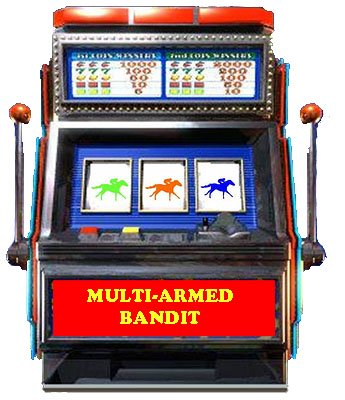
\includegraphics[scale=0.2]{multiarmed-bandit.jpg}
\end{center}
}

%%%%%%%%%%%%%%%%%%%%%%%%%%%%%%%%%%%%%%%%%%%%%%%%%%%%%%%%%%%%%%%%%%%%%%%%%%%%%%%%
\frame{
\frametitle{The bandits problem}
\scriptsize
\begin{itemize}
 \item If we knew the bandit with the largest probability, then always picking 
this bandit would yield the maximum winnings. So our task can be phrased as 
\highlt{Find the best bandit, and as quickly as possible}. 

\item The task is complicated by the stochastic nature of the bandits. A 
suboptimal bandit can return many winnings, purely by chance, which would make 
us believe that it is a very profitable bandit. Similarly, the best bandit can 
return many duds. Should we keep trying losers then, or give up? 

\item A more troublesome problem is, if we have found a bandit that returns 
\textit{pretty good} results, do we keep drawing from it to maintain our 
\textit{pretty good score}, or do we try other bandits in hopes of finding an 
\textit{even-better} bandit? This is the \highlt{exploration} vs. 
\highlt{exploitation} dilemma.
\end{itemize}
}

%%%%%%%%%%%%%%%%%%%%%%%%%%%%%%%%%%%%%%%%%%%%%%%%%%%%%%%%%%%%%%%%%%%%%%%%%%%%%%%%
\frame{ 
\frametitle{Exploration vs Exploitation}
\begin{itemize}
\item \keywd{Exploration}: Trying out different options to try and determine
the reward associated with the given approach (i.e. acquiring
more knowledge)
\ \\ \
\item \keywd{Exploitation}: Going with the approach that you believe to
have the highest expected payoff (i.e. optimizing decisions
based on existing knowledge)
\end{itemize}
}

%%%%%%%%%%%%%%%%%%%%%%%%%%%%%%%%%%%%%%%%%%%%%%%%%%%%%%%%%%%%%%%%%%%%%%%%%%%%%%%
\frame{
\frametitle{Multi-armed bandit applications go beyond A/B}
\footnotesize
\begin{itemize}
 \item \highlt{Internet display advertising}: What ad strategy will maximize 
sales? Naturally minimizing strategies that do not work (generalizes to A/B/C/D 
strategies)
 \item \highlt{Ecology}: How do the animals maximize its fitness w.r.t energy?
  \item \highlt{Finance}: which stock option gives the highest return, under 
time-varying return profiles.
  \item \highlt{Clinical trials}: a researcher would like to find the best 
treatment, out of many possible treatment, while minimizing losses. 
  \item \highlt{Psychology}: How does punishment and reward affect our 
behaviour? How do humans learn?
\end{itemize}
}

%%%%%%%%%%%%%%%%%%%%%%%%%%%%%%%%%%%%%%%%%%%%%%%%%%%%%%%%%%%%%%%%%%%%%%%%%%%%%%%
\frame{ 
\frametitle{Traditional A/B testing}

The process
\begin{itemize}
\item Start with pure exploration in which groups A and B are
assigned equal number of users
\item Once you think you have determined the better option, switch
to pure exploitation in which you stop the experiment and send
all users to the better performer
\end{itemize}

Potential issues
\begin{itemize}
 \item Equal number of observations are routed to A and B for a
preset amount of time or iterations
 \item Only after that preset amount of time or iterations do we stop
and use the better performer
 \item Waste time (and money!) showing users the site that is not
performing as well
\end{itemize}
}

%%%%%%%%%%%%%%%%%%%%%%%%%%%%%%%%%%%%%%%%%%%%%%%%%%%%%%%%%%%%%%%%%%%%%%%%%%%%%%%
\frame{
\frametitle{Multi-armed bandit solutions}
\begin{itemize}
\item Shows a user the site that you think is best most of the time
(exactly how is dictated by the strategy chosen)
\item As the experiment runs, we update the belief about the true
CTR (Click Through Rate)
\item Run for however long until we are satisfied the experiment has
determined the better site
\item Balances exploration and exploitation rather than doing only
one or the other
\end{itemize}
}

%%%%%%%%%%%%%%%%%%%%%%%%%%%%%%%%%%%%%%%%%%%%%%%%%%%%%%%%%%%%%%%%%%%%%%%%%%%%%%%
\frame{
\frametitle{Formalization}
\begin{itemize}
\item The model is given by a set of real distributions $B = {R_{1}, ..., 
R_{K}}$,
\item where each distribution is associated with the a reward delivered by
one of the $K \in N$ + levers.
\item We will let $\mu_{1}, ... , \mu_{K}$ be the mean values associated with 
these reward distributions.
\item The gambler plays one lever per round and observes the associated
reward. 
\item The goal is to maximize the sum of the collective rewards,
or alternatively minimize the agent’s \keywd{regret}
\end{itemize}
}

%%%%%%%%%%%%%%%%%%%%%%%%%%%%%%%%%%%%%%%%%%%%%%%%%%%%%%%%%%%%%%%%%%%%%%%%%%%%%%%
\frame{
\frametitle{Regret}
\begin{block}{}
The regret $p$ that an agent experiences after $T$ rounds is the
difference between the reward sum associated with an optimal
strategy and the sum of collected rewards
\end{block}

\begin{equation}
p = T \mu^{*} - \sum^{T}_{t=1} \hat{r}_{t}
\end{equation}

\begin{itemize}
 \item $\mu^{*}$ - is the maximal reward mean, $\mu^{*} = max_{k}\{\mu_{k}\}$
 \item $\hat{r}_{t}$ - is the reward at time t
 \item \keywd{Regret} is simply a measure of how often you choose a suboptimal 
bandit. We can think of this as the cost function we are trying to minimize
\end{itemize}
}

%%%%%%%%%%%%%%%%%%%%%%%%%%%%%%%%%%%%%%%%%%%%%%%%%%%%%%%%%%%%%%%%%%%%%%%%%%%%%%%
\frame{
\frametitle{A zero-regret strategy}

\begin{itemize}
 \item A zero-regret strategy is a strategy whose average regret per
round p/T tends to zero when the number of rounds played
tends toward infinity
 \item Interestingly enough, a zero-regret strategy does not guarantee
you will never choose a sub-optimal outcome, but rather
guarantees that, over time, you will tend to choose the optimal
outcome
\end{itemize}
}

%%%%%%%%%%%%%%%%%%%%%%%%%%%%%%%%%%%%%%%%%%%%%%%%%%%%%%%%%%%%%%%%%%%%%%%%%%%%%%%
\frame{
\frametitle{Epsilon-Greedy strategy}
\begin{itemize}
 \item Explore with some probability $epsilon$ (often 10\%)
 \item All other times we will exploit (i.e. choose the bandit with the
best performance so far)
 \item After we choose a given bandit we update the performance
based on the result.
\end{itemize}
}


%%%%%%%%%%%%%%%%%%%%%%%%%%%%%%%%%%%%%%%%%%%%%%%%%%%%%%%%%%%%%%%%%%%%%%%%%%%%%%%
\frame{
\frametitle{Other strategies}
\begin{block}{UCB1 - Upper confidence bound}
For the UCB1 algorithm we will choose whichever bandit that has
the largest value. 
\end{block}
\vspace{1cm}
\begin{block}{softmax}
For the softmax algorithm we will choose the bandit randomly in
proportion to its estimated value.
\end{block}
}

%%%%%%%%%%%%%%%%%%%%%%%%%%%%%%%%%%%%%%%%%%%%%%%%%%%%%%%%%%%%%%%%%%%%%%%%%%%%%%%
\section{Bayesian Bandits}
\subsection{}

%%%%%%%%%%%%%%%%%%%%%%%%%%%%%%%%%%%%%%%%%%%%%%%%%%%%%%%%%%%%%%%%%%%%%%%%%%%%%%%
\frame{
\frametitle{Bayesian Bandits}
The Bayesian bandit algorithm involves modeling each of our bandits
with a beta distribution with the following shape parameters:
\begin{itemize}
 \item $\alpha$ = 1 + number of times bandit has won
 \item $\beta$ = 1 + number of times bandit has lost
\end{itemize}

We will then take a random sample from each bandit’s distribution
and choose the bandit with the highest value.
}

%%%%%%%%%%%%%%%%%%%%%%%%%%%%%%%%%%%%%%%%%%%%%%%%%%%%%%%%%%%%%%%%%%%%%%%%%%%%%%%
\frame{
\frametitle{Bayesian Bandits}
\scriptsize
\begin{block}{} 
There are also many approximately-optimal solutions which are quite 
good. One of the few solutions that can scale incredibly well. The solution is 
known as \keywd{Bayesian Bandits}.
\end{block}
\vspace{1cm}
These strategies are an example of \keywd{online algorithms} because they are 
continuously-being-updated, aka \keywd{reinforcement 
learning algorithm}. The algorithm starts in an ignorant state, where it knows 
nothing, and begins to acquire data by testing the system. As it acquires data 
and results, it learns what the best and worst behaviors are (in this case, it 
learns which bandit is the best).
}


%%%%%%%%%%%%%%%%%%%%%%%%%%%%%%%%%%%%%%%%%%%%%%%%%%%%%%%%%%%%%%%%%%%%%%%%%%%%%%%
\frame{
\begin{itemize}
 \item Like in a normal multi-arm problem, an agent must choose
between arms during each iteration
 \item Before making the choice, the agent sees a d-dimensional
feature vector (context vector), associated with the current
iterations state
 \item The agent uses the context vector as well as the history of past
rewards to choose the arm to play in the current iteration
 \item Over time, the aim is for the agent to learn how the context
vectors relate to the associated rewards so as to pick the
optimal arm
\end{itemize}
}

%%%%%%%%%%%%%%%%%%%%%%%%%%%%%%%%%%%%%%%%%%%%%%%%%%%%%%%%%%%%%%%%%%%%%%%%%%%%%%%
\frame{
\frametitle{Summary}
\begin{itemize}
\item The problem originated with a gambler standing in front of a
row of slot machines (referred to as \textit{one-armed bandits})
\item The agent has to decide which machines to play, how many
times to play each machine, and it which order
\item Each bandit will provide a reward from a unknown distribution
\item Objective is to maximize the sum of rewards earned through a
series of lever pulls
\item There are several classes of fairly optimal solutions 
\end{itemize}
}

%%%%%%%%%%%%%%%%%%%%%%%%%%%%%%%%%%%%%%%%%%%%%%%%%%%%%%%%%%%%%%%%%%%%%%%%%%%%%%
\frame{ 
\frametitle{Check-in questions}
\begin{block}{}
\highlt{Core questions}
\begin{enumerate} 
 \item Can you contrast \keywd{exploration} vs \keywd{exploitation}
 \item Can you use plain English to explain what \keywd{regret} means in this context?
 \item Cay you explain any of the following strategies: Epsilon-Greedy, Softmax, or UCB1 in your own words.
 \item What is the Bayesian Bandit strategy and how is it an example of \keywd{online learning}?
 \end{enumerate}
\end{block}
}


%%%%%%%%%%%%%%%%%%%%%%%%%%%%%%%%%%%%%%%%%%%%%%%%%%%%%%%%%%%%%%%%%%%%%%%%%%%%%%
\frame[allowframebreaks]{  
\frametitle{References}
\begin{tiny} \bibliography{pp.bib}
\bibliographystyle{apalike}         % Style BST file
\end{tiny}
}

\end{document}